% !Mode:: "TeX:UTF-8"
% !TEX program  = xelatex

% \documentclass{cumcmthesis}
\documentclass[withoutpreface,bwprint]{cumcmthesis} %去掉封面与编号页,电子版提交的时候使用。


\usepackage[framemethod=TikZ]{mdframed}
\usepackage{url}   % 网页链接
% \usepackage{subcaption} % 子标题
\title{穿越沙漠路径规划的宽度优先搜索模型}

\begin{document}

    \maketitle
    \begin{abstract}
        本文针对穿越沙漠最优路径规划问题,基于图论、宽度优先搜索、博弈论纳什均衡理论,建立了数学模型,为游戏参与者提供了不同情境下的最优策略。

        我们使用一个五元组\((d,p,f,w,m)\)来描述游戏参与者所处的状态,其中\(d,p,f,w,m\)分别表示游戏参与者所在日期、所处位置、所带食物,所带水和所带资金。游戏开始时游戏参与者处在\((0,1,0,0,10000)\)节点,目标是在\(d\leq\)限定时间内到达\(p=\)终点,同时使\(m\)尽可能的大。状态之间的转移包括前进、停留、挖矿和购买物资四种。

        在第一问中,我们用起点、村庄、矿山和终点构成加权连通图,每条边的权值对应于两个顶点之间的最短路线,我们证明了在已知全部天气时这样的加权图可以代替原地图,减少了节点数,简化了计算。

        在一名玩家且已知全部天气情况时,我们可以具体表示出每一步状态转移对应的水、食物和资金的消耗,利用宽度优先搜索,从只包含\((0,1,0,0,10000)\)的队列开始拓展,
        % 每次从队头取出一个节点,按照状态转移方法拓展出所有可行节点,将他们放入原队列队尾,不断重复直到队列为空。利用宽度优先搜索,我们
        可以找到所有能够从起点在限制时间内到达终点的路径,将他们放入一个以到达终点所保留的资金进行比较的优先队列,就能得到最优策略。

        在第二问中,我们采用估值函数来确定最佳策略,对于游戏中的每一天,已知当天的天气情况,我们都可以计算,对于每一种接下来的选择:停留、购物、挖矿、前进到每一个邻格,分别计算在这种选择下,以后所有天都是晴朗天气和都是高温天气时限制时间内走到终点的最大持有的资金,取一个平均值作为这种选择的预期收益,再以预期收益最大的那种选择作为最优策略。这种计算的方法中,计算终点持有资金时之后的天气情况已经全部设定了,就可以利用第一问的方法去计算,只需要把当前位置当作“不能再以基准价格购物的起点”就行。

        % 在第三问中,我们

\keywords{宽度优先搜索\quad 图搜索\quad 规划模型\quad 纳什均衡}
\end{abstract}

%目录  2019 明确不要目录,我觉得这个规定太好了
%\tableofcontents

%\newpage

\section{问题重述}

穿越沙漠问题是一个在约束条件下求最优解的问题,具体来说,指在给定的地图上,玩家在游戏开始时获得一定的初始资金,可以在起点购买一定数量的水和食物,然后从起点出发,穿过沙漠抵达终点。在穿越沙漠中,玩家所携带的水和食物不能呢超越其最大背负重量,但必须大于等于当天的消耗,从而不至于渴死或者饿死。穿越途中会遇到不同的天气,也可以在矿山获得资金,或者在村庄购买资源,抵达终点之后也可以退回多余的水和食物。游戏要求在规定的时间到达终点,在终点拥有的资金则多多益善。

我们需要建立数学模型解决如下具体问题:

\subsection{问题一}
只有一名玩家,游戏开始时,游戏时间内每天天气情况就全部已知,在此条件下求解一个最优策略,使得到达终点时持有最多的资金。

\subsection{问题二}
只有一名玩家,玩家只知道当天的天气情况,求解一个最优策略,使得玩家能根据当天的天气情况选择当天的行动,使得到达终点时持有最多的资金。


\subsection{问题三}


\section{问题分析}

\subsection{问题一的分析}
问题一中游戏全程的天气情况都是已知的,那么对于每一步的状态转移,我们都能直接计算出这一步状态转移所消耗的资产、水和食物。这样,从起点这一初始状态出发,按照状态转移模型中的条件,我们就可以通过宽度优先搜索,直接搜索出所有起点到终点的完整路径,并找出其中到达终点退还物资后,保留的资产最多的一条路径,这就是我们要求的最优路径。

\subsection{问题二的分析}
相比于问题一,只知道当天的天气情况,我们没法将从当天所在位置开始每种能在时间限制内到达终点的方案,以及到达终点后保留的资金具体的计算出来,但我们可以通过假定天气情况序列来解决这一难题。对于游戏中的每一天,已知当天的天气情况,我们都可以计算,对于每一种接下来的选择:停留、购物、挖矿、前进到每一个邻格,分别计算在这种选择下,以后所有天都是晴朗天气和都是高温天气时限制时间内走到终点的最大持有的资金,取一个平均值作为这种选择的预期收益,再以预期收益最大的那种选择作为最优策略。这种计算的方法中,计算终点持有资金时之后的天气情况已经全部设定了,就可以利用第一问的方法去计算,只需要把当前位置当作“不能再以基准价格购物的起点”就行。

\subsection{问题三的分析}

% \section{基本假设}

% \begin{enumerate}
%     \item 纳什均衡假设。对于多个游戏参与者而言,当
% \end{enumerate}

\section{变量说明}

\begin{table}[!htbp]
    \caption{符号说明}\label{tab:001} \centering
    \begin{tabular}{ccc}
        \toprule[1.5pt]
        符号 & 意义 & 单位\\
        \midrule[1pt]
        $d$ & 当前日期 & \\
        $p$ & 所在的区域编号 & \\
        $f$ & 所带的食物 & 箱\\
        $w$ & 所带的水 & 箱\\
        $m$ & 所带的资金 & 元\\
        \bottomrule[1.5pt]
    \end{tabular}
\end{table}

\section{模型的建立与求解}

我们从图搜索模型的三要素:状态描述、状态转移模型、最终目标来描述这个数学模型。

\subsection{状态的描述}
首先我们讨论状态的描述。我们可以用一个五元组\((d,p,f,w,m)\)来描述当前所处的状态,其中各个符号意义如表\ref{zt},则起始状态可以描述为\((0,1,0,0,10000)\)
\begin{table}[!htbp]
    \caption{五元组中的符号说明}\label{tab:001} \centering
    \begin{tabular}{ccc}
        \toprule[1.5pt]
        符号 & 意义 & 单位\\
        \midrule[1pt]
        $d$ & 当前日期 & \\
        $p$ & 所在的区域编号 & \\
        $f$ & 所带的食物 & 箱\\
        $w$ & 所带的水 & 箱\\
        $m$ & 所带的资金 & 元\\
        \bottomrule[1.5pt]
    \end{tabular}
    \label{zt}
\end{table}

\subsection{状态的转移模型}
接着我们讨论状态的转移模型。根据题目给出的规则,从每个状态出发,有四种可行的去向:
\begin{enumerate}
    \item 购买物资,这种转移发生在第0天的起点或者第若干天的村庄,并消耗掉对应资产,\(m\)减小,\(f,w\)相应发生变化。
    \item 前进,从某个地点(起点、村庄或者矿山),前进到另一个地点(村庄、矿山或者终点),此过程所花费的时间,\(\geq\)两个地点间最短路径长度,\(\leq\)截止日期--从该地点出发的时间--终点和到达地点的最短路径长度,以保证能在截止日期前到达终点。在时长超过最短路径的前进过程中会有停留,此时优先在这段时间里基础消耗量最大的天气里停留,然后是在基础消耗量次大的天气里停留,最后是基础消耗量最小的天气里停留。并且,消耗掉对应水和食物,\(w,f\)减小。
    \item 停留,在某个地点(起点、村庄或者矿山)停留,此过程所花费的时间,\(\geq\)1天,\(\leq\)截止日期--终点和该地点的最短路径长度,以保证能在截止日期前到达终点。并且,消耗掉对应水和食物,\(w,f\)减小。
    \item 挖矿,在到达矿山的后一天挖矿,此过程所花费的时间,\(\geq\)1天,\(\leq\)截止日期--终点和该矿山的最短路径长度,以保证能在截止日期前到达终点。并且,消耗掉对应水和食物,\(w,f\)减小。
\end{enumerate}
此外,任意一个可行的状态都必须满足\(f\geq 0\)且\(w\geq 0\),不能渴死或者饿死。

\subsection{最终目标}

游戏的最终目标是在\(d\leq\)限定时间内到达\(p=\)终点,同时使\(m\)尽可能的大。在第三问中,涉及到\(n\)个游戏参与者,此时要\(\sum_{i=1}^n m_i\)尽可能的大。

\subsection{对第一问的宽度优先搜索模型}

我们可以很容易地证明,在天气情况全部已知的同一段时间内,从地图的A处到达B处,走最短路径并把多余的时间全部用于在途中停留,这样做所消耗的资源和资金,小于等于走次短路径全程走路所消耗的,所以我们可以忽略次短路径。因此,我们可以先对地图做一些简化。

沙漠的地图可以抽象为一张无向连通图,我们可以通过宽度优先搜索(BFS)来确定起点、村庄、矿山、终点之间的最短路径,就可以把有数十个节点的地图\ref{dt}简化为只有几个顶点的加权连通图\ref{jianhua}。简化过程如图\ref{jianhuaguocheng}所示。

\begin{figure}
    \centering
    \begin{minipage}[c]{0.45\textwidth}
        \centering
        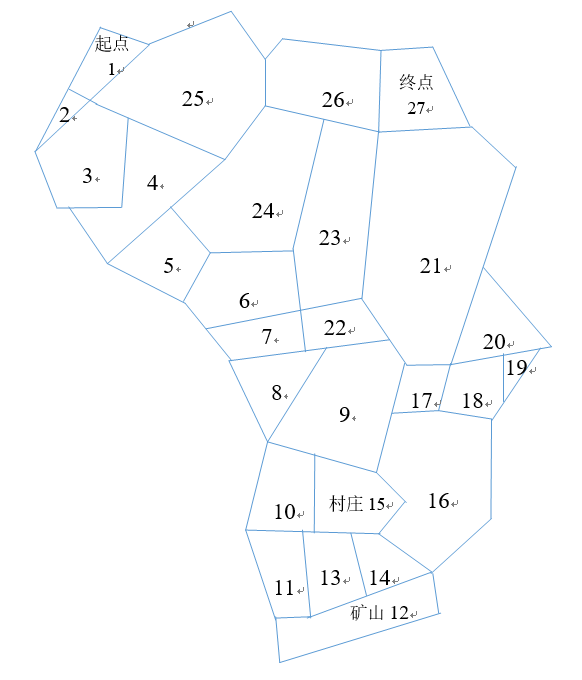
\includegraphics[width=0.95\textwidth]{figures/dt.png}
        \subcaption{第一关地图}
        \label{dt}
    \end{minipage}
    \begin{minipage}[c]{0.45\textwidth}
        \centering
        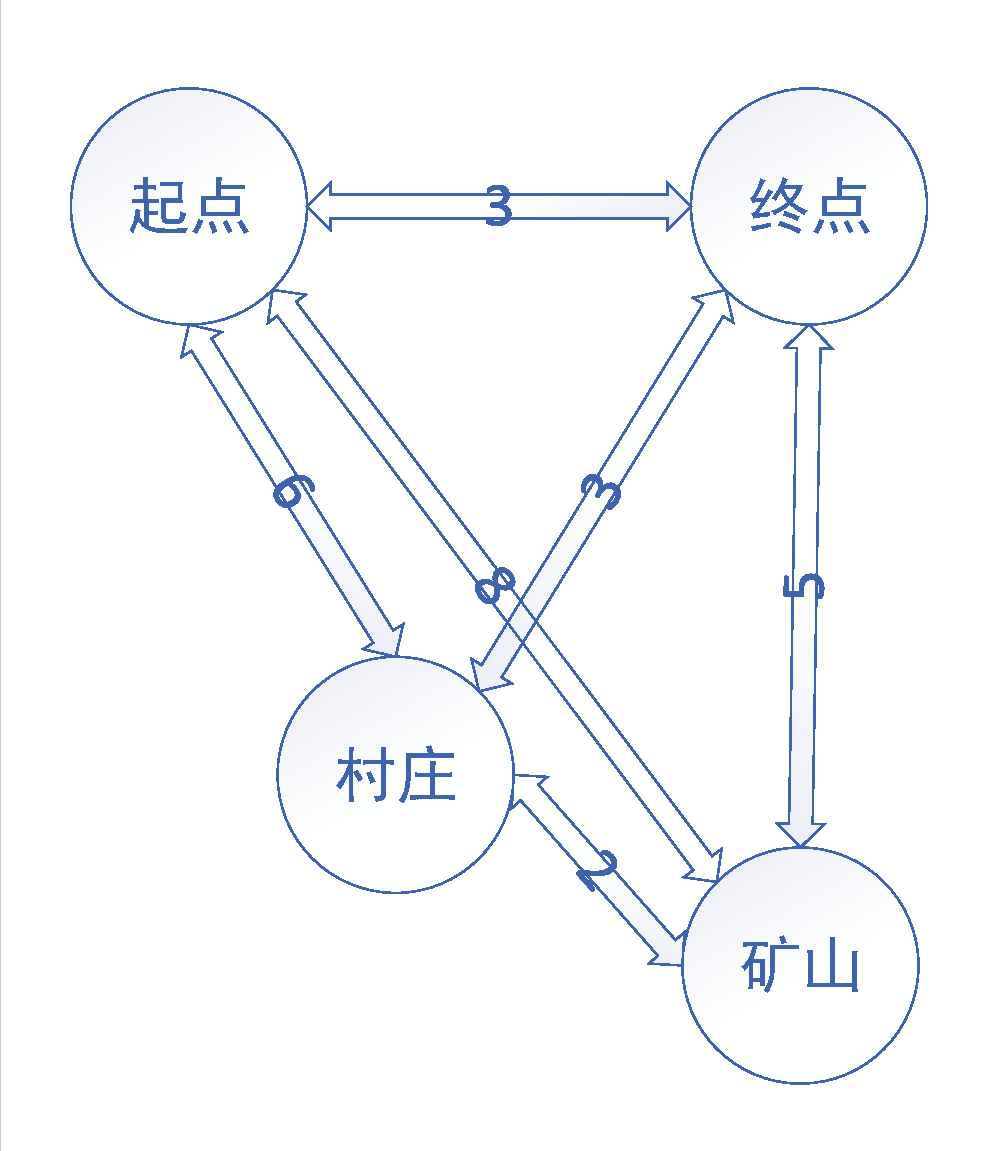
\includegraphics[width=0.95\textwidth]{figures/jianhua.pdf}
        \subcaption{简化后加权图}
        \label{jianhua}
    \end{minipage}
    \caption{用最短路径简化地图}
    \label{jianhuaguocheng}
\end{figure}



\section{参考文献与引用}

%参考文献
\begin{thebibliography}{9}%宽度9
    % \bibitem[1]{liuhaiyang2013latex}
    % 刘海洋.
    % \newblock \LaTeX {}入门\allowbreak[J].
    % \newblock 电子工业出版社, 北京, 2013.
    \bibitem{mathematical-modeling}
    全国大学生数学建模竞赛论文格式规范 (2020 年 8 月 25 日修改).
    \bibitem{latexstudio} \url{https://www.latexstudio.net}
\end{thebibliography}

\newpage
%附录
\begin{appendices}

\section{程序}

\begin{lstlisting}[language=matlab]

\end{lstlisting}

\end{appendices}

\end{document} 